\documentclass[a4paper,11pt,hidelinks]{article}
%\usepackage[a-1b]{pdfx}
\usepackage{hyperref}

\usepackage{subfiles}
\usepackage{epsfig}
\usepackage{plain}
\usepackage{setspace}
%\usepackage{minted}
\usepackage{listings}

\usepackage{mdframed}
\usepackage{caption}
\usepackage{color}
\usepackage{amsmath}
\usepackage{amsthm}
\usepackage{amssymb}
\usepackage{amsfonts}
\usepackage{mathabx}
\usepackage{tcolorbox}
\usepackage{multicol}
\usepackage[english]{babel}
\usepackage[left=2cm,right=2cm,top=2cm,bottom=1.8cm]{geometry}
\usepackage{titlesec} 
\usepackage[utf8x]{inputenc} 

\hypersetup{colorlinks=true, urlcolor=blue}

\captionsetup{
  justification=centering,
  singlelinecheck=false,
  font=small,labelfont=bf,labelsep=space}

\begin{document}

\pagestyle{plain} 

\begingroup

\renewcommand{\cleardoublepage}{}
\renewcommand{\clearpage}{}

\titleformat{\section}
{\normalfont\Large\bfseries}{\thesection}{1em}{}


\renewcommand{\lstlistingname}{Code}%
\renewcommand{\lstlistlistingname}{List of \lstlistingname s}

\definecolor{codeBackground}{rgb}{0.9, 0.9, 0.9}

% Code environment
\lstnewenvironment{code}[1]{
    \mdframed[%
        backgroundcolor=codeBackground,
        shadow=false,
        linecolor=black!40,
        linewidth=2pt,
        topline=false,
        rightline=false,
        leftline=false
    ]%
    \lstset{%
        moredelim=**[is][\color{blue}]{**}{**},
        moredelim=**[is][\color{teal}]{.-}{-.},
        moredelim=**[is][\color{gray}]{||}{||},
        frame=single,
        framerule=0pt,
        basicstyle=\ttfamily,
        columns=fullflexible
    }%
}{% Spacing between and after caption + before end of mdframed
    \vspace{-1em}
    \endmdframed
    \vspace{-0.5em}
    \captionsetup{type=lstlisting}
    \caption{#1}
    \vspace{1.5em}
    \ignorespaces
}


\newpage

\title{Internetworking exercise}
\author{Offensive Technologies 2021 \\    
Matteo Franzil \texttt{<matteo.franzil+github@gmail.com>}}
\maketitle

\section{Solution}

This exercise was solved as the following. First, I inspected the created nodes from the web interface:

\begin{code}{Code found in the DeterLAB web interface.}
pc162	||NWworkstation1||	pc3060	Ubuntu-EDU	up [...]
pc177	||NWrouter||	pc3060	Ubuntu-EDU	up [...]
pc179	||ISrouter||	pc3060	Ubuntu-EDU	up [...]
pc181	||SWrouter||	pc3060	Ubuntu-EDU	up [...]
pc201	||SWworkstation1||	pc3060	Ubuntu-EDU	up [...]
\end{code}

The grey names are the names of the nodes of the experiment in which we're going to install our network configuration.

Second, I ssh-ed into the control plane and uploaded the script file (\verb=working-demo.sh=). The script file was written by combining data from the exercise page on DeterLAB (\url{https://www.isi.deterlab.net/file.php?file=/share/shared/Internetworking}), which provides network configuration information step-by-step, into a single, whole file. Indeed, the first time I executed the exercise, I first did it step by step, but kept the executed commands and then condensed it into the script.

First, the script pings \url{/share/shared/Internetworking/showcabling} in order to retrieve the configuration set up by DeterLAB (the so known "wired connections):

\begin{code}{Obtaining the network cabling setup.}
$ /share/shared/Internetworking/showcabling Franzil-Iworking offtech

NWworkstation1 eth5 <- is "wired" to -> NWrouter eth5
NWrouter eth3 <- is "wired" to -> ISrouter eth2
ISrouter eth1 <- is "wired" to -> SWrouter eth5
SWworkstation1 eth3 <- is "wired" to -> SWrouter eth3
\end{code}   

These are then filtered and saved as PATH variables in order to keep them at hand.

Then, I chose some subnets to apply to the nodes. This is the network I obtained:

\begin{code}{Simplified diagram of the network.}
 NW-workstation
       | .1
[10.0.100.0/28]
       | .2
      NW-r
       | .1
[2.0.100.0/28]
       | .2
      IS-r
       | .1
[3.0.100.0/28]
       | .2
      SW-r
       | .1
[10.0.400.1/28]
       | .2
 SW-workstation
\end{code}

Only \verb=.1= and \verb=.2= IPs were assigned, with the logic that southbound (i.e. facing south on the DeterLAB exercise page and in the above diagram) interfaces would get \verb=.1=, northbound interfaces would get \verb=.2=. So as an example, the northwest workstation has a single southbound interface, and is thus numbered \verb=10.0.100.1=. This is also reflected in the script by the interface names saved in the variables.

Then, the script proceeds to apply the network configuration as required the exercise (IP addresses; routing; blocking of private addresses; NAT; port-forwarding). I decided to use the newer \verb=ip= commands instead of the \verb=ifconfig= ones as it is now recommended to use the formers.

For five times, the script saves the configuration to a \verb=sh= file and, using the ability to share the home folder between DeterLAB nodes, does an \verb=ssh= to each machine and applies it as a superuser (thus avoiding a sudo for each command).

\section{Example outputs}

This section contains some example outputs presented during the execution of the exercise. For example, this is what happens when pinging the two workstation with private address blocking enabled:

\begin{code}{TCPdump with private address blocking.}
root@nwrouter:~# tcpdump -nnti eth3 icmp
tcpdump: verbose output suppressed, use -v or -vv for full protocol decode
listening on eth3, link-type EN10MB (Ethernet), capture size 262144 bytes
IP 10.0.100.1 > 10.4.100.2: ICMP echo request, id 17109, seq 51, length 64
IP 10.0.100.1 > 10.4.100.2: ICMP echo request, id 17109, seq 52, length 64
IP 10.0.100.1 > 10.4.100.2: ICMP echo request, id 17109, seq 53, length 64
IP 10.0.100.1 > 10.4.100.2: ICMP echo request, id 17109, seq 54, length 64
\end{code}

On the other hand, this is when NAT is enabled and the workstations ping each other using their router's IP:

\begin{code}{Pinging each other with NAT.}
IP 2.0.100.1 > 3.0.100.2: ICMP echo request, id 19365, seq 391, length 64
IP 3.0.100.2 > 2.0.100.1: ICMP echo reply, id 19365, seq 391, length 64
IP 2.0.100.1 > 3.0.100.2: ICMP echo request, id 19365, seq 392, length 64
IP 3.0.100.2 > 2.0.100.1: ICMP echo reply, id 19365, seq 392, length 64
IP 2.0.100.1 > 3.0.100.2: ICMP echo request, id 19365, seq 393, length 64
IP 3.0.100.2 > 2.0.100.1: ICMP echo reply, id 19365, seq 393, length 64
\end{code}

Furthermore, some screenshots are included in the next pages.

\begin{figure}
  \centering
  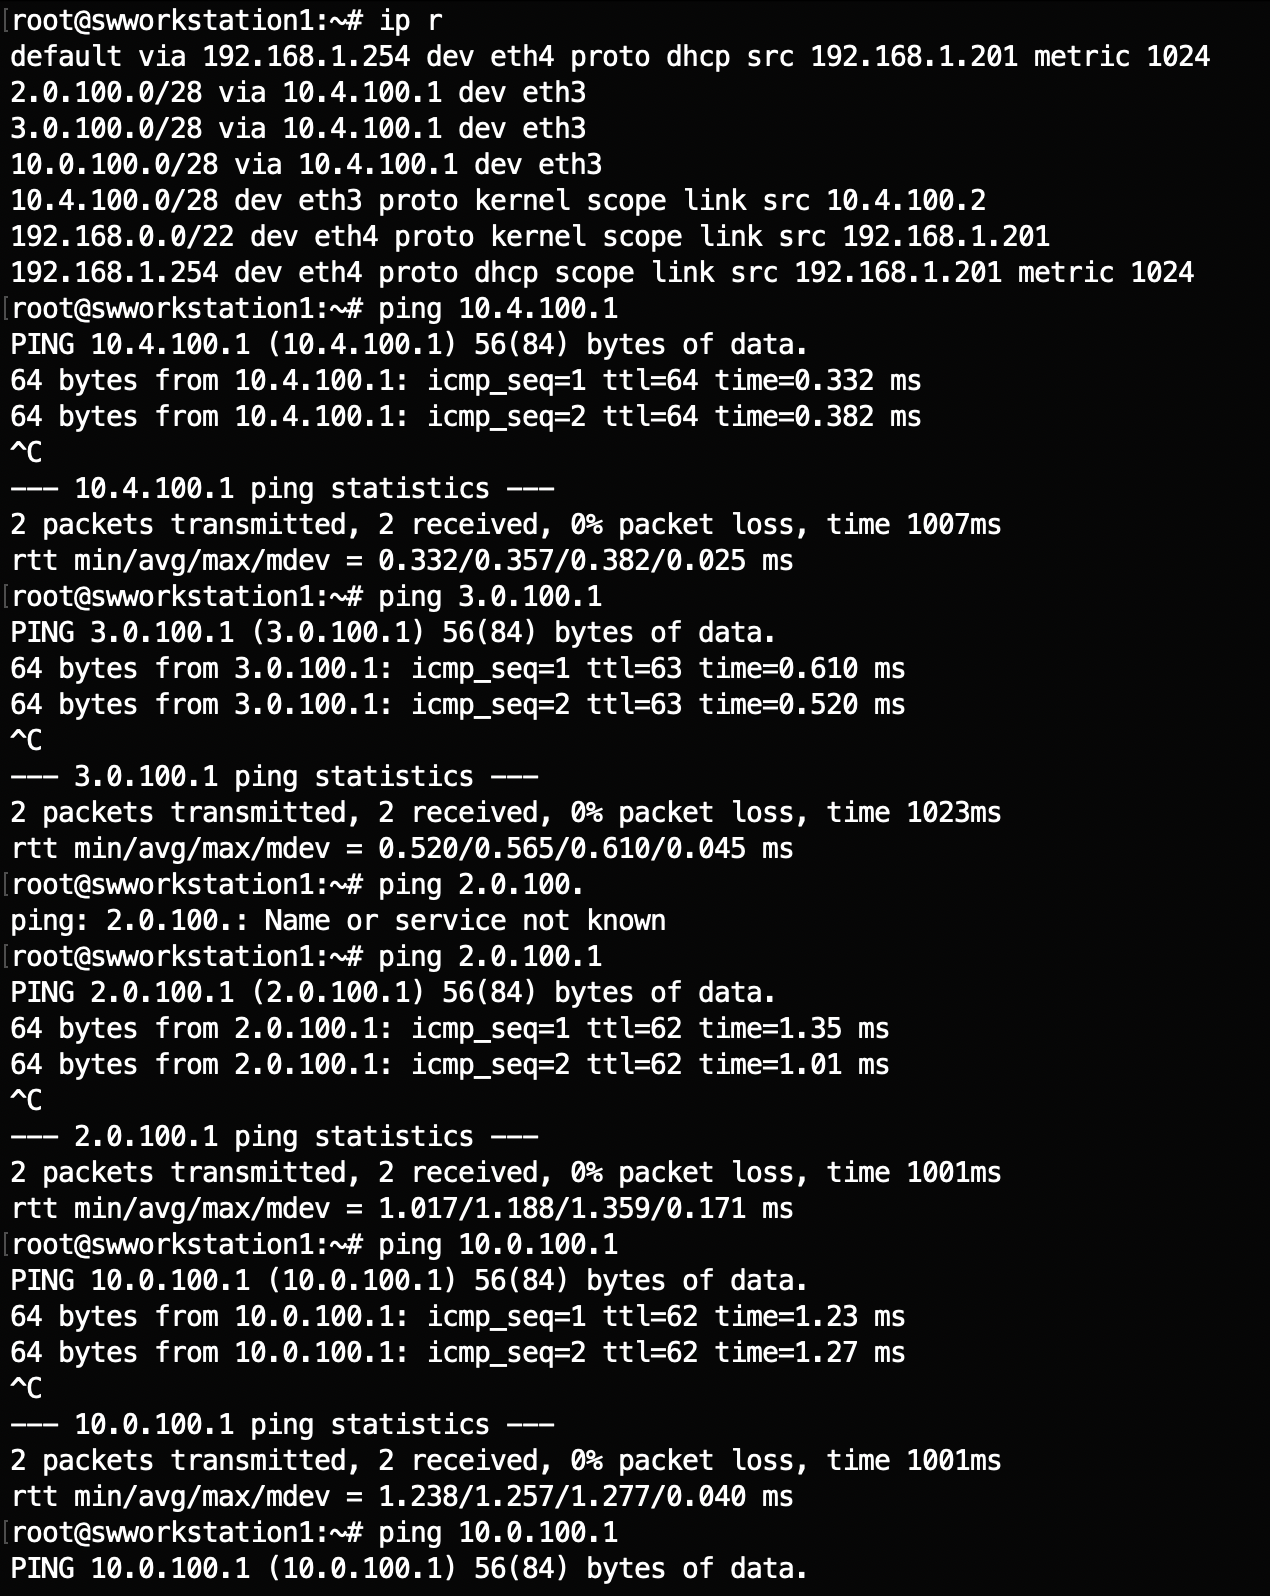
\includegraphics[width=\textwidth]{../drawable/ping-result.png}
  \caption{Example of pings passing through to all other four machines from the southwest workstation.}
\end{figure}

\begin{figure}
  \centering
  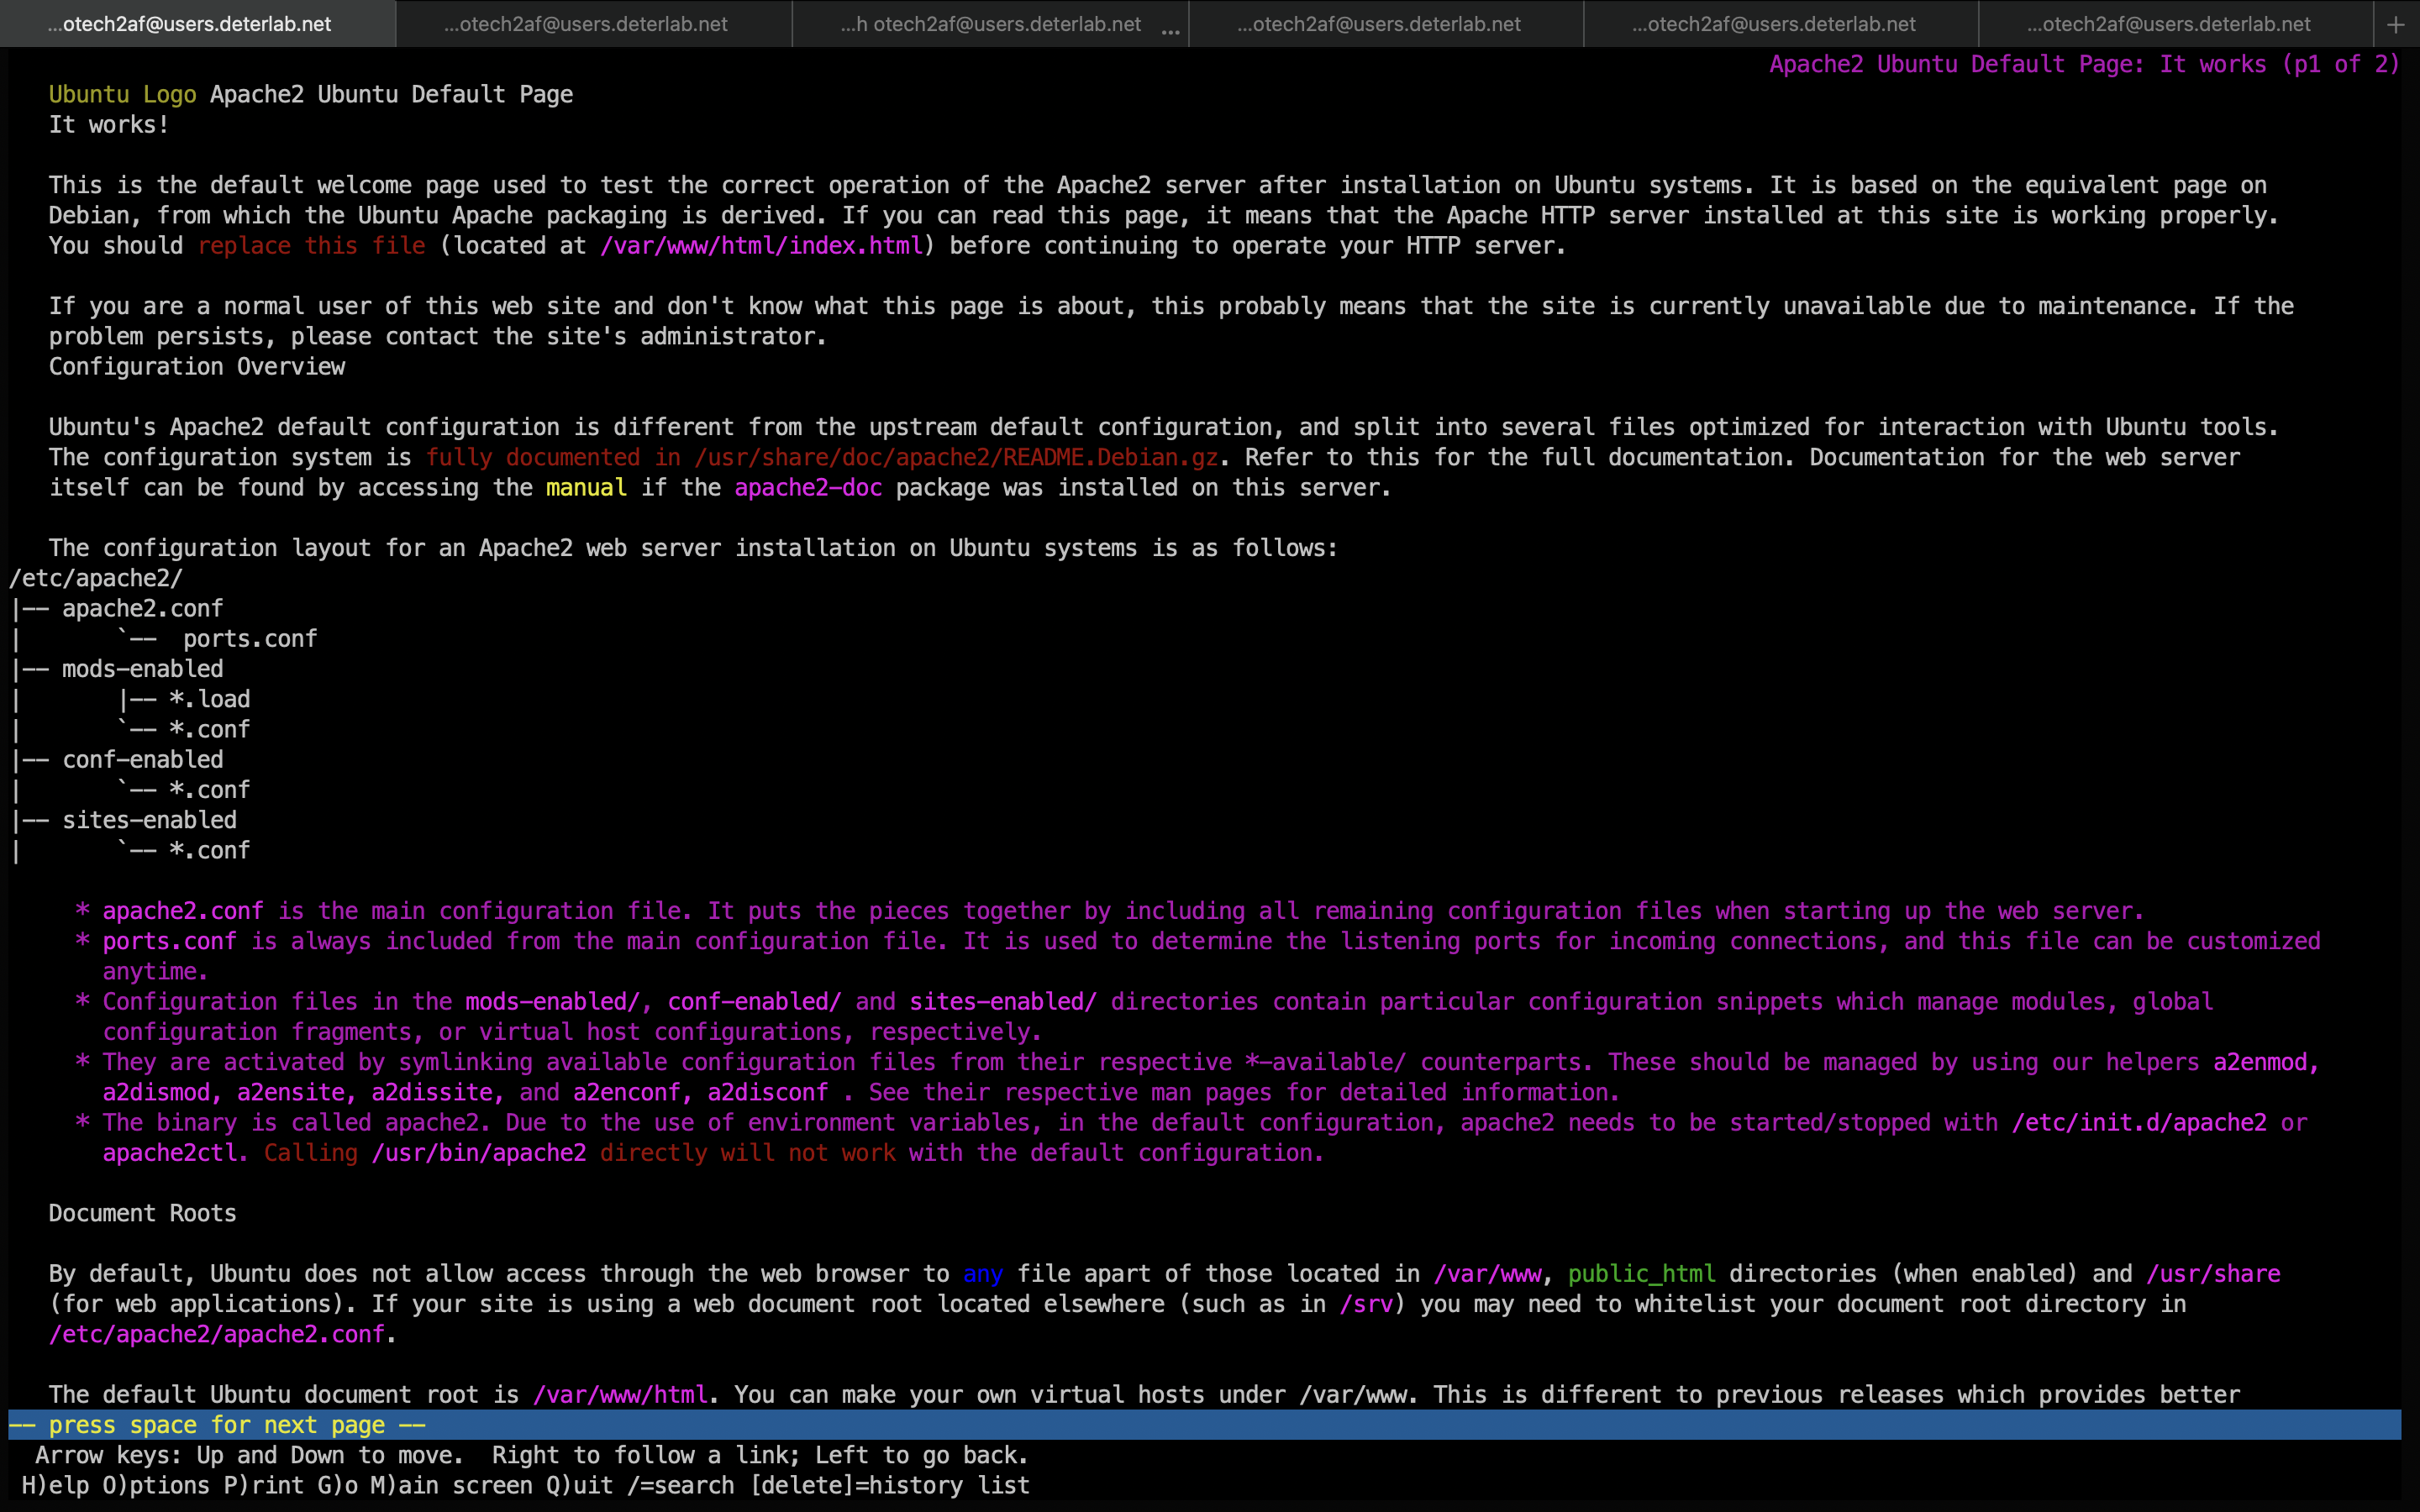
\includegraphics[width=\textwidth]{../drawable/lynx-result.png}
  \caption{Final result of the exercise, yielding the Apache web server visualized with the Lynx web browser.}
\end{figure}

\begin{figure}
  \centering
  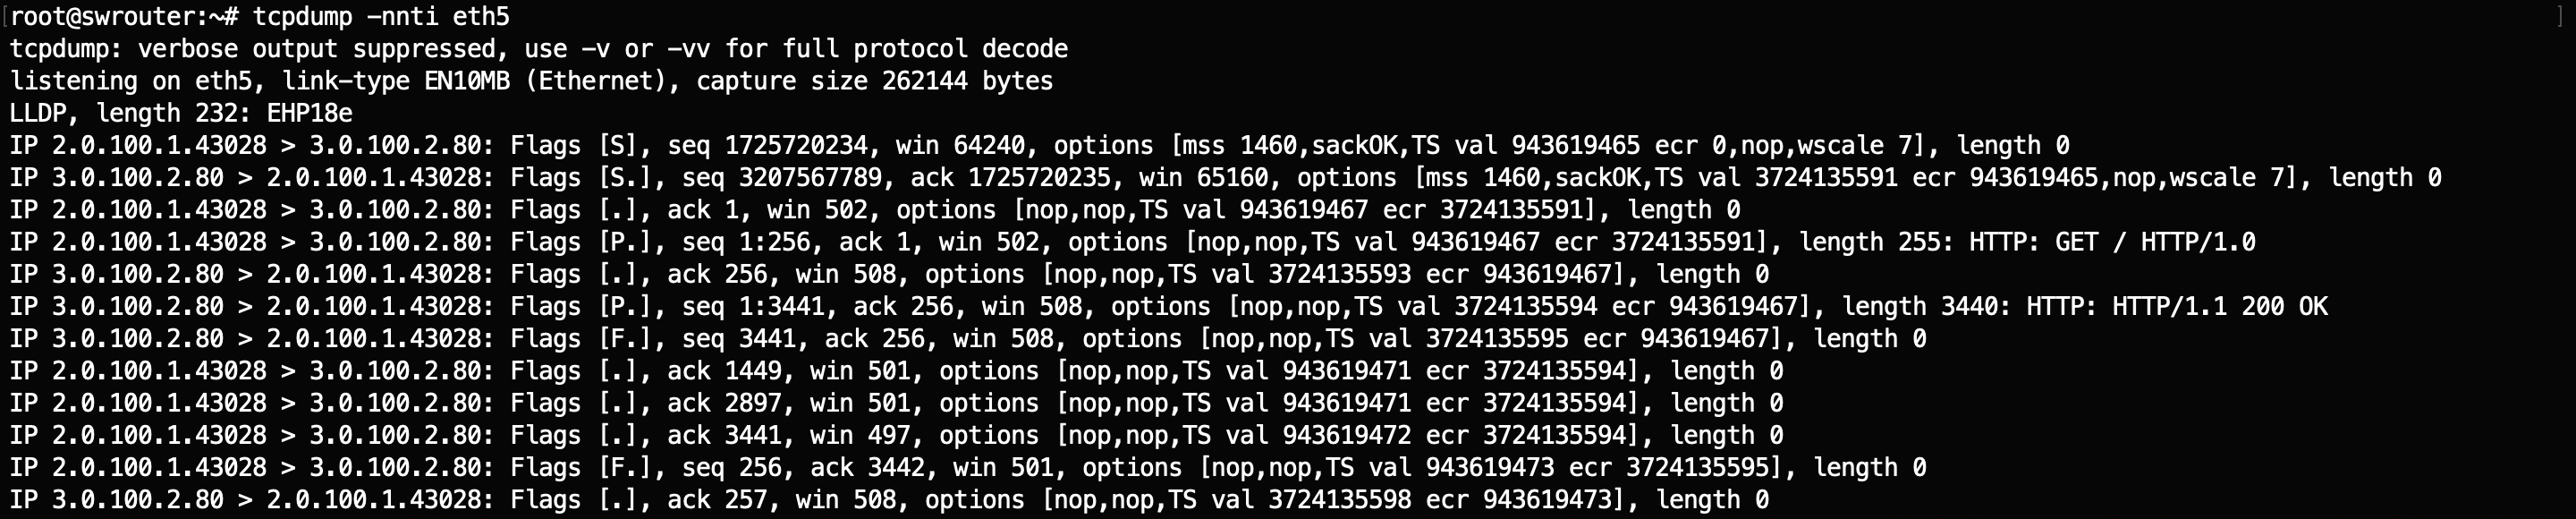
\includegraphics[width=\textwidth]{../drawable/tcpdump-nat-result.png}
  \caption{TCPdump result of the Lynx-Apache connection.}
\end{figure}

\endgroup

\end{document}
